%\clearpage
%\clearpage
%\input{../introduction/problem.tex}
%%\clearpage
%\input{../introduction/goal.tex}
%%\clearpage
%\input{../introduction/mission.tex}
\section{Introduction}
\todo{Grundlagen}

	\begin{enumerate}
		\item \textbf{Acceleration with constant force]} 0.15 seconds with 16N
		\item \textbf{Parabelflight} Until the parachute ist open at a velocity of $-20^m/_s$
		\item \textbf{Parachute flight} Constant velocity of $-20^m/_s$
	\end{enumerate}

	\begin{eqnarray}
		v\left( t\right)  &= v_0 + a * t\\
		s\left( t\right)  &= s_0 + v_0 * t + 0.5 * a * t^2
	\end{eqnarray}
	
	
	
	
\section{Model}


	\begin{figure}[H]
		\centering
		\includegraphics[width=0.7\textwidth]{figures/overview.png}
		\caption{Overview of the simulink model.}
		\label{fig:overview}
	\end{figure}


\section{Simulation}	
	
	\begin{figure}[H]
		\centering
		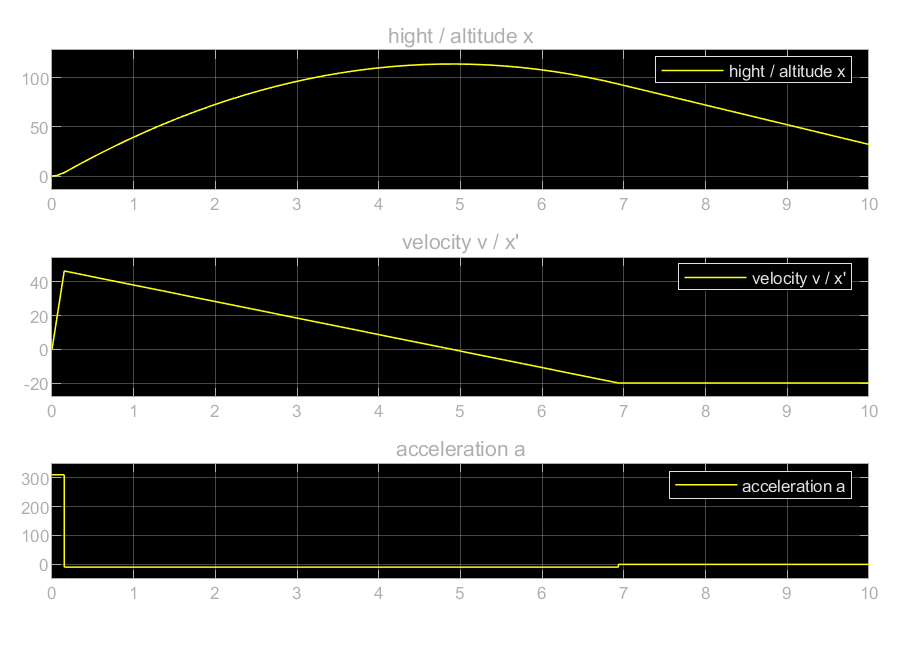
\includegraphics[width=0.7\textwidth]{figures/scope.eps}
		\caption{Scope from the Simulation.}
		\label{fig:scope1}
	\end{figure}
	
	
	
	

	\begin{lstlisting}
		clear all; clc; close all;
		
		%%
		% g inverted
		m=0.05; g=-9.81; tEngine=0.15; Force=16; vChute=-20; Dt=0.01; 
		clear t v h 
		n=1; 
		t(n)=0; v(n)=0; h(n)=0; t(2)=0;
		
		%%
		% Segment 1 
		a1=(Force-m*g)/m; 
		while (t(n) < tEngine) &&  (n < 50000) 
		n=n+1; 
		t(n)=t(n-1)+Dt; 
		v(n) =a1 *t (n) ; 
		h(n) =0.5*a1*t(n)^2;
		end;
		v1=v(n); h1=h(n); t1=t(n);
		
		% Segment 2
		while v(n)>=vChute && n<50000
		n=n+1;
		t(n)=t(n-1)+Dt;
		v(n)=v1-g*(t(n)-t1);
		h(n) =h1+v1 * (t(n)-t1 )-0.5*g* (t (n)-t1)^2;
		end
		v2=v(n); h2=h(n); t2=t(n);
		
		% Segment 3
		while h(n)>0 && n<50000
		n=n+1;
		t(n)=t(n-1)+Dt;
		v(n)=vChute;
		h (n) =h2+vChute* (t(n)-t2) ;
		end
		
		%%
		subplot(1,2,1)
		plot(t,h,t2,h2, 'ro', t1, h1, 'r+')
		xlabel('Time [s]');
		ylabel('Hight [m]');
		subplot(1,2,2)
		plot(t,v,t2,v2, 'ro', t1, v1, 'r+')
		xlabel('Time [s]');
		ylabel('Velocity [m]');
	\end{lstlisting}